\section{Results}

\subsection{RQ1}


1. Fig: x-axis is models, y-axis are hallucinated package absolute number and relative hallucination percentage.



\begin{figure}[!t]
    \centering
    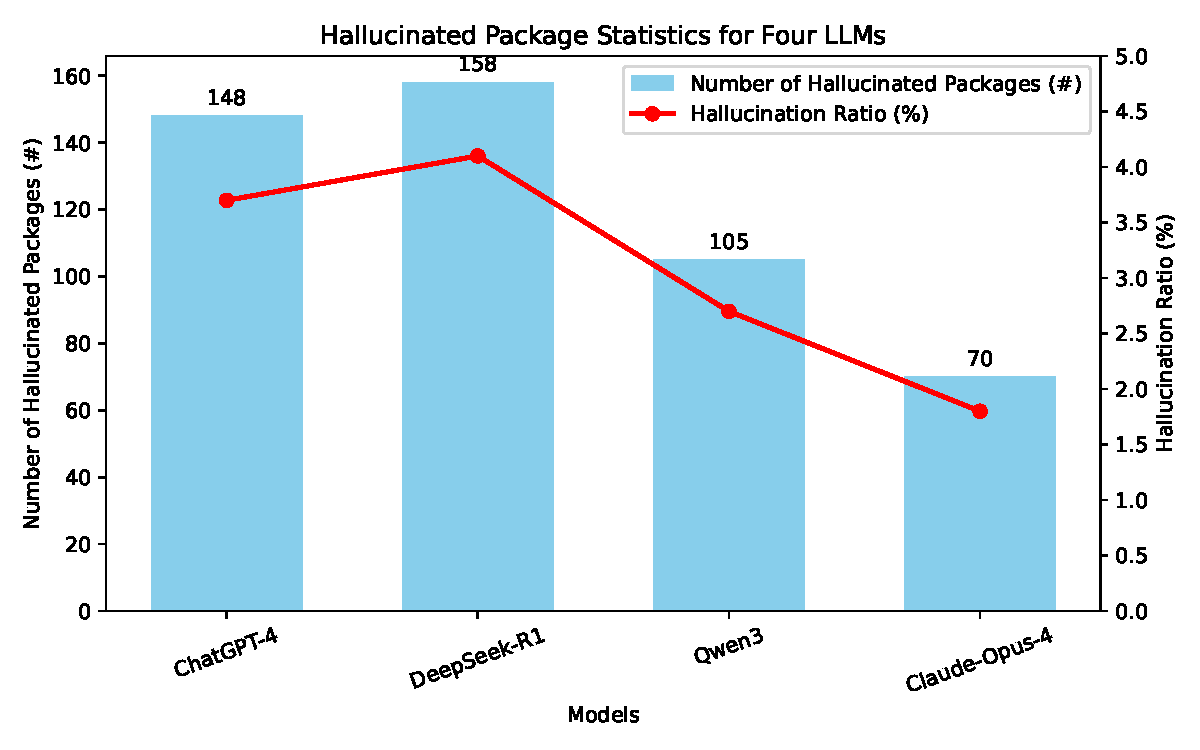
\includegraphics[width=0.45\textwidth]{fig/RQ1-hallucinated-packages.pdf}
    \vspace{-10pt}
    \caption{The number and ratio of hallucinated packages generated by four LLMs.}
    \label{fig:hallucinated-packages}
\end{figure}



2. Fig: x-axis is hallucinated packages ranked by their hallucination times among models, y-axis is the hallucination number.



\begin{figure}[!t]
    \centering
    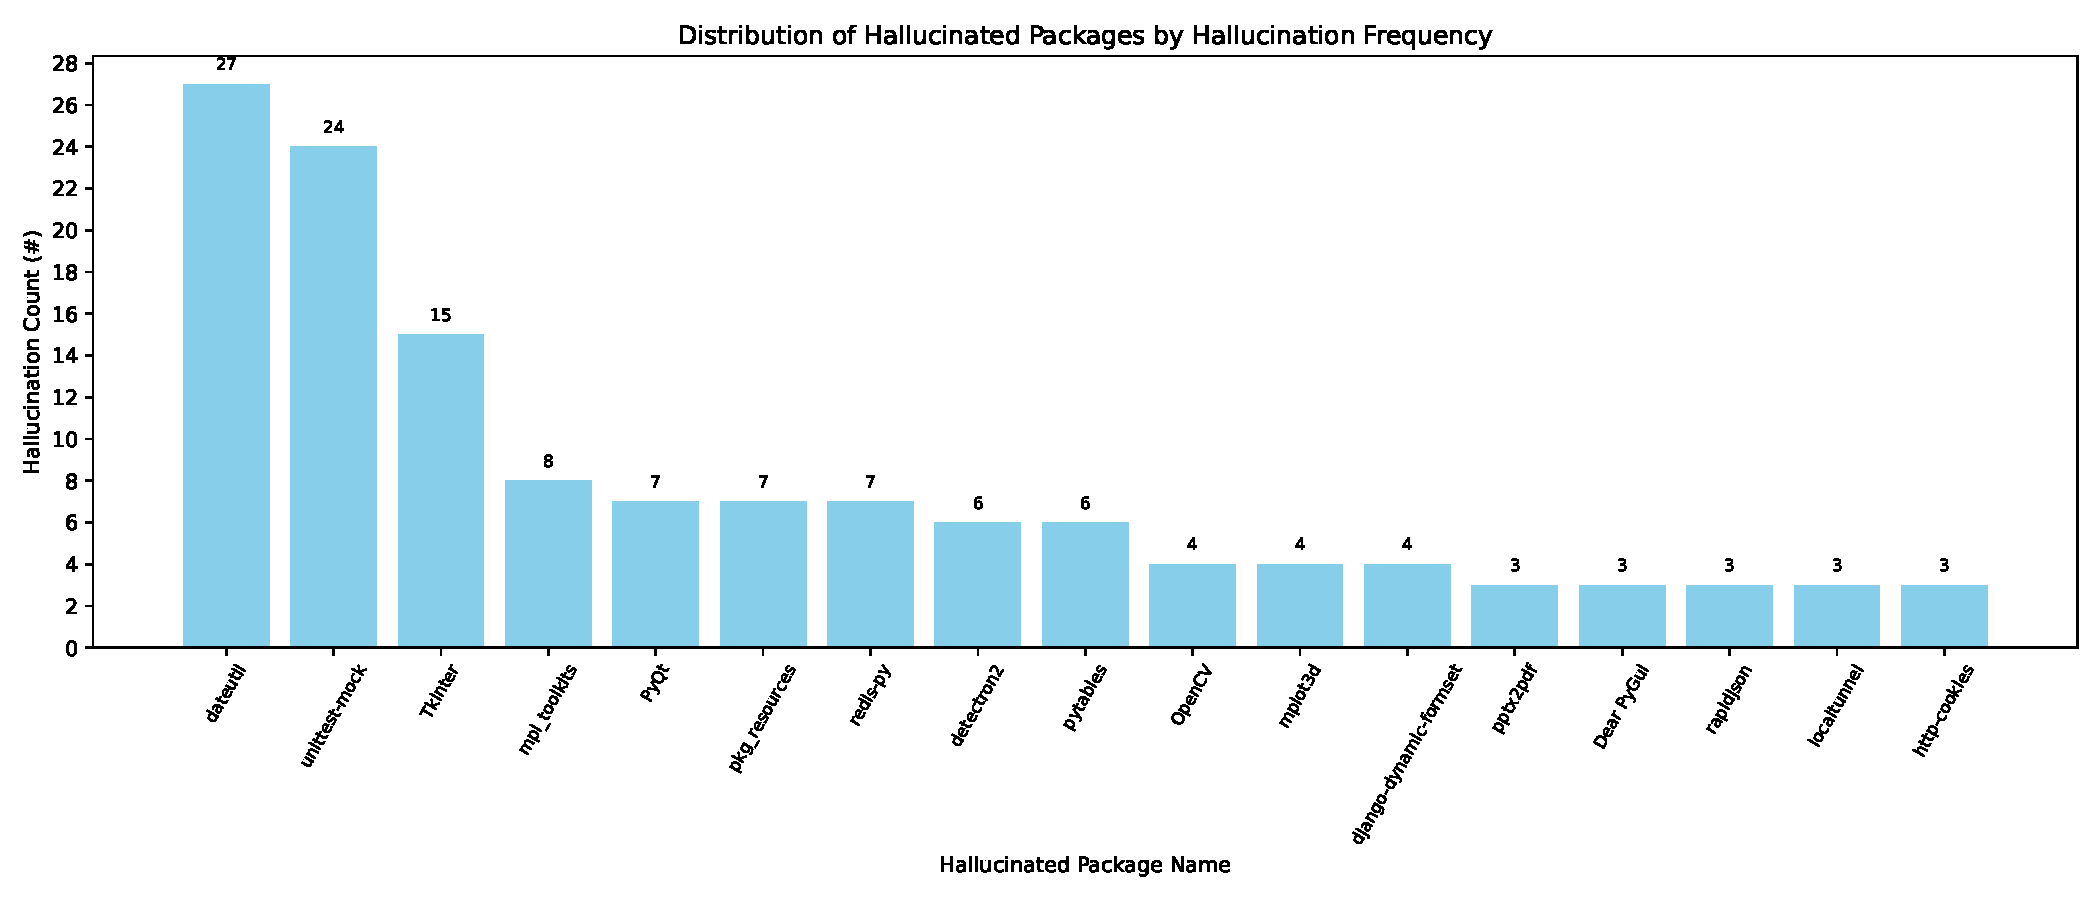
\includegraphics[width=0.48\textwidth]{fig/RQ1-hallucinated-frequency.pdf}
    \vspace{-10pt}
    \caption{Distribution of hallucinated packages by hallucination frequency.}
    \label{fig:hallucinated-frequency}
\end{figure}


\begin{figure}[!t]
    \centering
    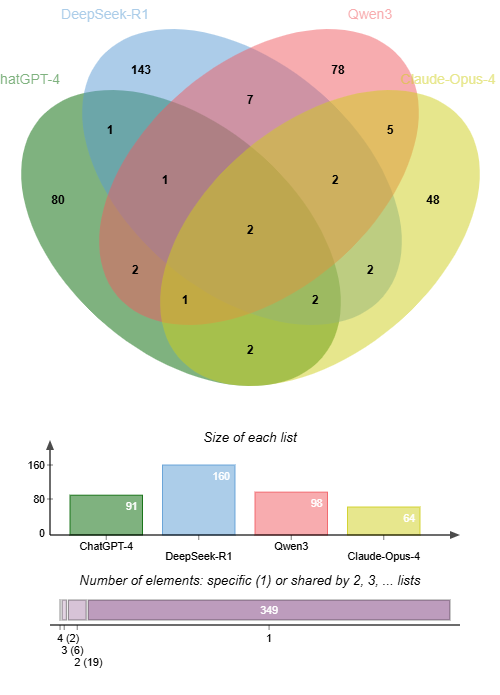
\includegraphics[width=0.48\textwidth]{fig/RQ1-hallucination-vnn.png}
    \vspace{-10pt}
    \caption{Venn diagram of hallucinated package overlaps among LLMs.}
    \label{fig:hallucination-vnn}
\end{figure}


\subsection{RQ2}

% repeat the above process and figure 

1. Package name characteristics.

    1.1 Syntactic analysis 
    1.2 Package domain analysis 

2. Analysis on questions that cause hallucinated package name.

\subsection{RQ3}

x-axis is time, y-axis is total download times, and average download number.

\begin{figure}[!t]
    \centering
    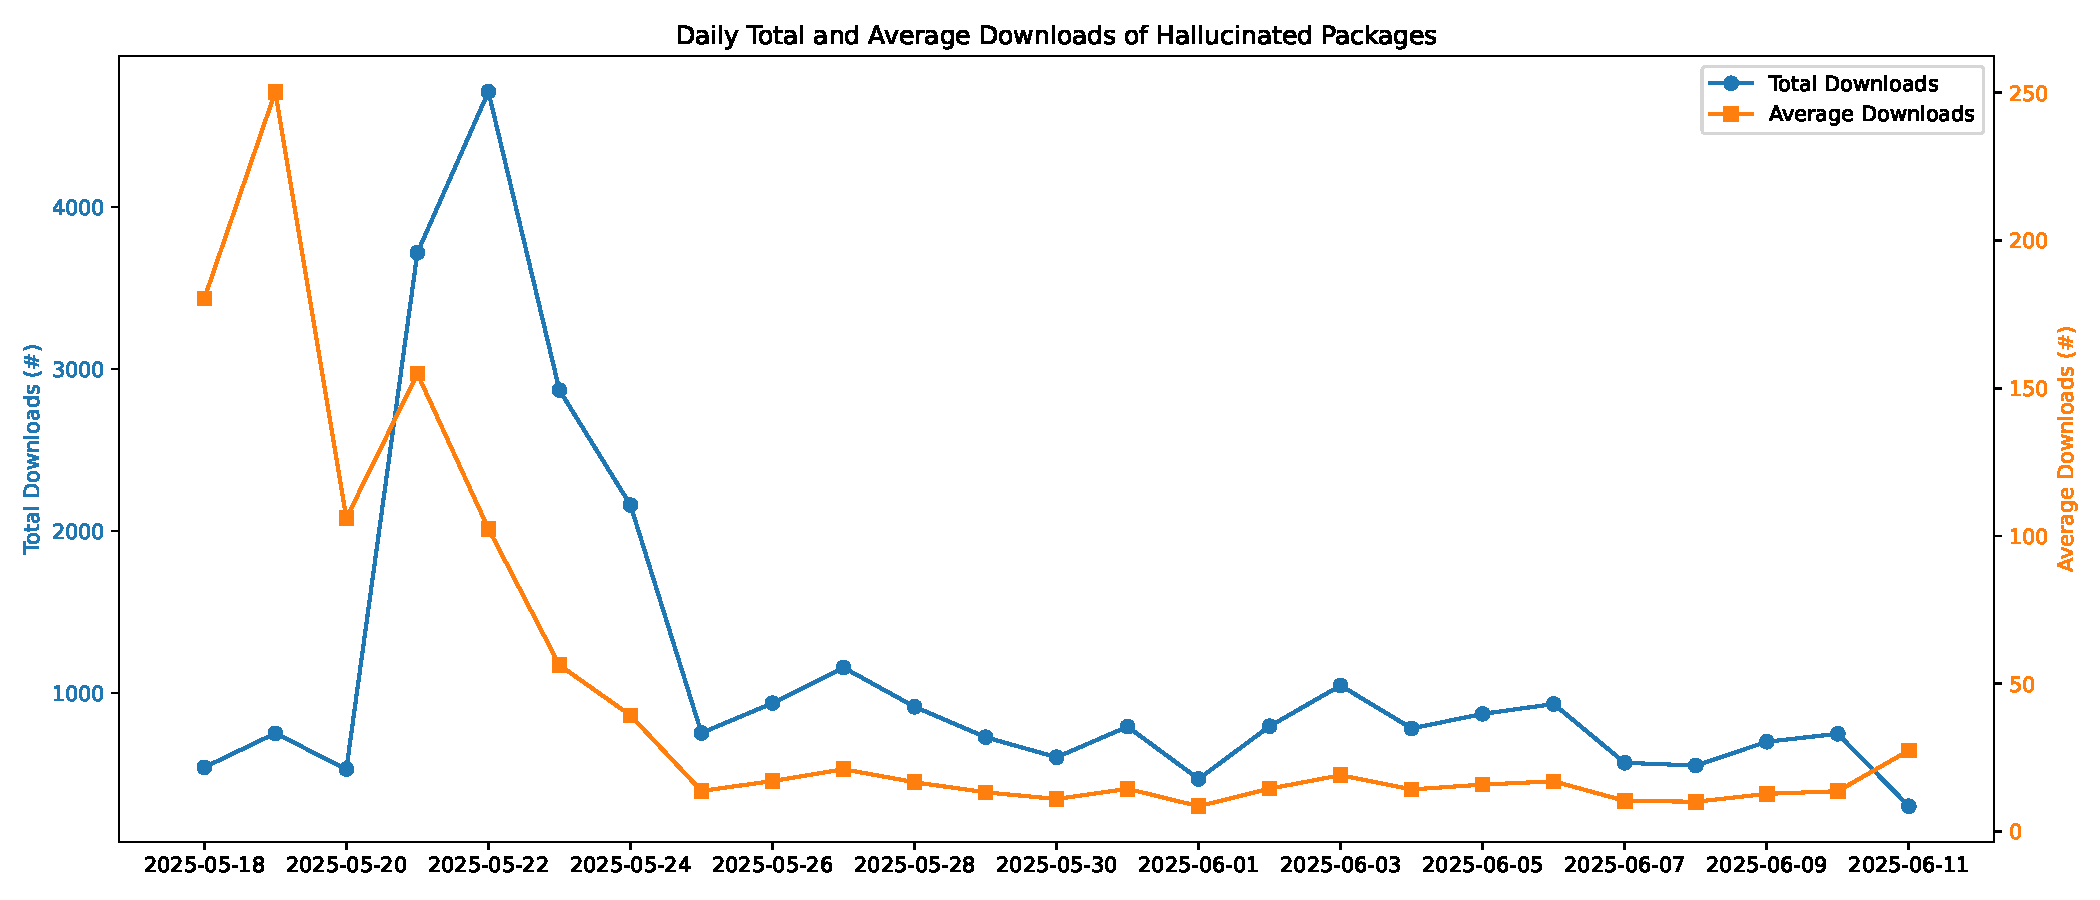
\includegraphics[width=0.48\textwidth]{fig/RQ3-hallucinated-downloads.pdf}
    \vspace{-10pt}
    \caption{Daily total and average downloads of hallucinated packages.}
    \label{fig:hallucinated-downloads}
\end{figure}


\begin{figure}[!t]
    \centering
    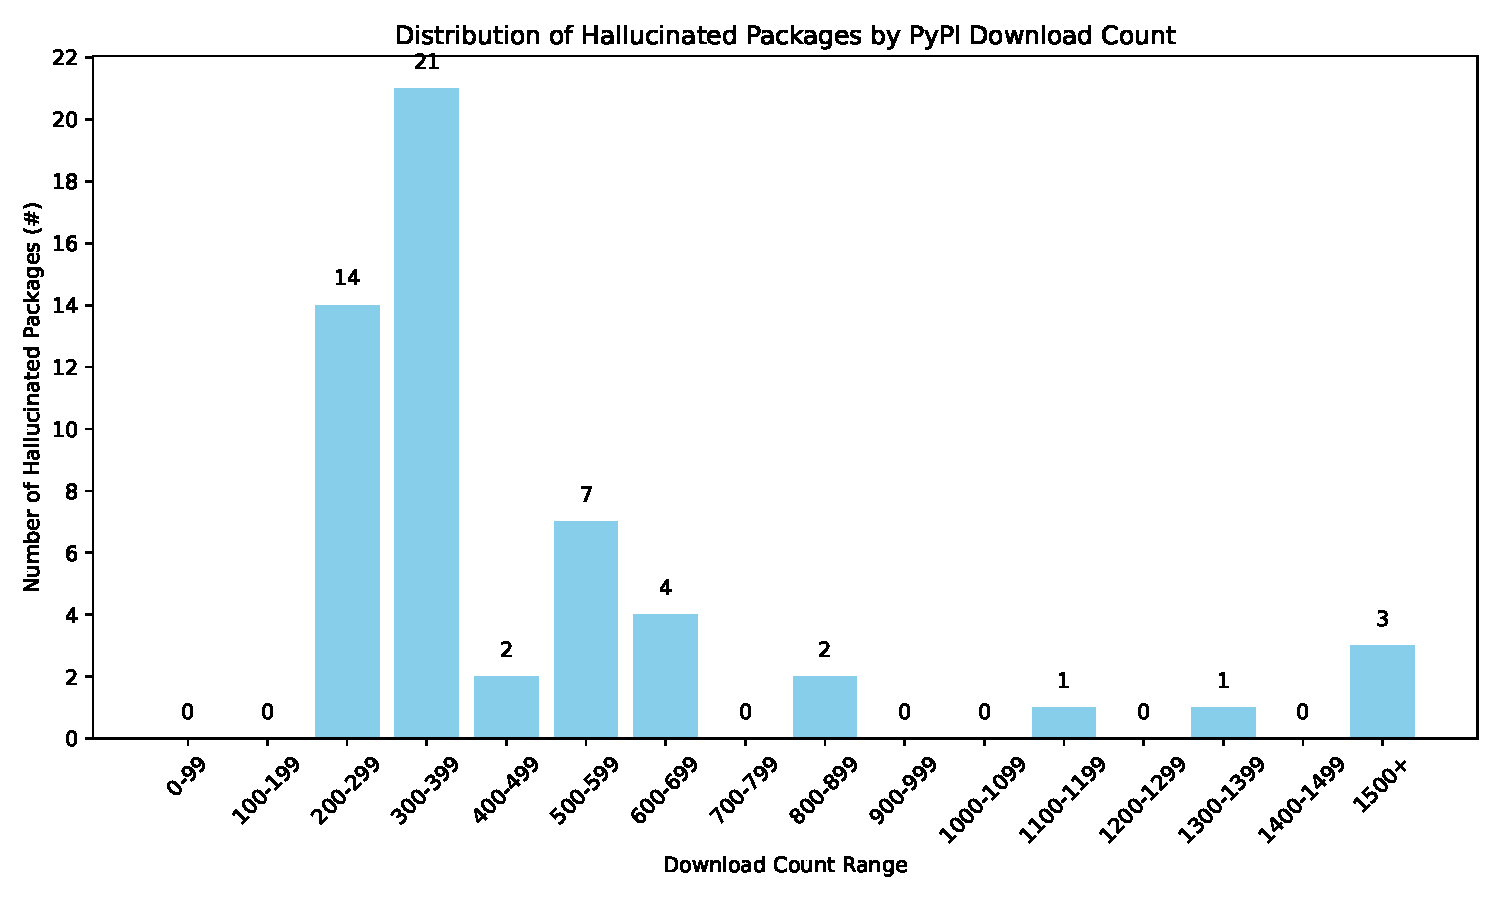
\includegraphics[width=0.45\textwidth]{fig/RQ3-hallucinated-downloads-2.pdf}
    \vspace{-10pt}
    \caption{Distribution of hallucinated packages by total PyPI downloads.}
    \label{fig:hallucinated-downloads-2}
\end{figure}


\todo{TODO fig. download numbers with regard to package names}

\subsection{RQ4}

Put Table, illustrate characteristics.



% Conclusion:

% 1. 如何提问可以使得幻觉率更低？
% 2. 幻觉的包，在不同domain/包名上表现的分布差异？
% 3. rewrite之后，不同rewrite形式，幻觉率不同
\begin{table*}[!t]
    \centering
    \footnotesize
    \caption{Feature Categories of Hallucinated PyPI Package Names}
    \label{tab:hallucination_features}
    \begin{tabular}{p{4cm}p{10cm}c}
    \toprule
    \textbf{Feature Category} & \textbf{Example Package Names} & \textbf{Count} \\
    \midrule
    PyPI Submodules & \texttt{mpl\_toolkits}, \texttt{mplot3d}, \texttt{gridfs}, \texttt{pkg\_resources}, \texttt{sklearn-base}, \texttt{django-forms} & 6 \\
    Function/Usage Names & \texttt{odeint}, \texttt{django-contenttypes} & 2 \\
    Misspelled Packages & \texttt{urlib3}, \texttt{shutilwich}, \texttt{maze-solvers} & 3 \\
    Fabricated Based on Real PyPI Packages & \texttt{django-classy-views}, \texttt{flask-autocomplete} & 20+ \\
    Import Name Mismatch & \texttt{MySQLdb}, \texttt{yaml}, \texttt{dateutil} & 3 \\
    Old Package Names & \texttt{pytest-capturelog} & 1 \\
    Standard Library Names & \texttt{email-parser}, \texttt{osrandom}, \texttt{redirect-stdout}, \texttt{BytesIO} & 4 \\
    Legacy Stdlib Names & \texttt{Tkinter} & 1 \\
    Colloquial or Informal Names & \texttt{redis-py}, \texttt{pyqt}, \texttt{opencv} & 3 \\
    Derived from Technical Terms & \texttt{translate-api}, \texttt{pycapsule-api}, \texttt{manifestin} & 3 \\
    Platform / C Library / Tools & \texttt{zeromq}, \texttt{OpenSSL}, \texttt{package\_control}, \texttt{h2oai}, \texttt{tastypie}, \texttt{sslsplit} & 6 \\
    \bottomrule
    \end{tabular}
    \end{table*}
    
